\documentclass[12pt]{standalone}

\usepackage{tikz}

\begin{document}
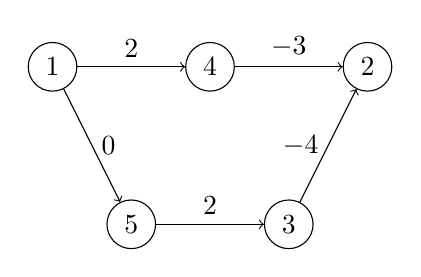
\begin{tikzpicture}

\begin{scope}[every node/.style={circle,draw}]
    \node (1) at (0,2) {1};
    \node (2) at (4,2) {2};
    \node (3) at (3,0) {3};
    \node (4) at (2,2) {4};
    \node (5) at (1,0) {5};
\end{scope}

\path[->]
    (1) edge node[above] {$2$} (4)
        edge node[right] {$0$} (5)
    (4) edge node[above] {$-3$} (2)
    (5) edge node[above] {$2$} (3)
    (3) edge node[left] {$-4$} (2);

\end{tikzpicture}
\end{document}
